\documentclass[11pt,letterpaper]{article}

\usepackage{graphicx}
\usepackage[margin=1in]{geometry}
\usepackage{amsmath}
\usepackage[T1]{fontenc}
\usepackage[utf8]{inputenc}
\usepackage{authblk}
\usepackage{fancyhdr}
\usepackage{lastpage}
\usepackage[parfill]{parskip}
\usepackage{subcaption}

\pagestyle{fancyplain}
\fancyhf{}
\fancyfoot[R]{\footnotesize Page \thepage\ of \pageref{LastPage}}

\renewcommand{\headrulewidth}{0.0pt} % No header rule
\renewcommand{\footrulewidth}{0.4pt} % Thin footer rule

\begin{document}

\title{Visual Discovery of Communication Patterns in Email Networks}

\author[ ]{Benjamin Bengfort}
\author[ ]{Konstantinos Xirogiannopoulos}
\affil[ ]{Department of Computer Science}
\affil[ ]{University of Maryland}
\affil[ ]{\textit{\{bengfort,kostasx\}@cs.umd.edu}}

\date{April 6, 2015}

\maketitle

\section*{Introduction}

In the age of social networks, it is very popular to analyze Twitter and Facebook to detect relationships and communities and to discover how information flows between groups. However, both Facebook and Twitter are examples of "performed" social networks, that is, because a user has full control over who he or she "friends" or "follows" they can artificially create a persona that they wish the outside world to perceive them as. In fact, it has been well studied that expressions of taste typically exclude the most critical groups to communication flows, and that social networks are merely the expressions of performed taste \cite{liu_social_2007}.

Email, on the other hand, is used in every facet of modern life and typically includes and aggregate facets of ourselves that would otherwise be segregated - for example, professional and personal personas. Because we spend so much time writing, reading, and responding to email it has become integrated into a communication fabric that far exceeds other media that may get more analytical attention like text messaging or social networks. Email therefore can be seen to embed a natural communication network, from which we can extract rich insights about actual communications and influences within a single ego network - that is the email \textt{mbox} of a single user - without the bias of taste performance.

If a user could be equipped with some understanding of the natural communication flow in a non-performed communication domain, we believe it would lead to more effective communication. In this paper, we will explore the analysis of two personal email networks, one from each of the authors, where one network is extremely large in terms of the number of nodes (emails participating) and the other network is extremely large in terms of the number of edges (cliquish, highly connected email). In particular, we hope to show that if a user can visualize their own networks, they will better understand the dynamic nature of their communication in terms of key players, communities, and gaps in communication - and be better able to respond to information in a meaningful way.

In this paper we will use Gephi \cite{gephi_gephi-open_2010} to visualize email networks that have been extracted from \texttt{mbox} files via a Python tool written by the authors called \texttt{tribe}, which serializes the network into GraphML \cite{brandes_graph_2010}. Gephi has been used for visual exploration and mapping of networks \cite{bastian_gephi:_2009} and includes many features for the statistical analysis of small to medium networks \cite{mcsweeney_gephi_2009}. Work of note includes an analysis of dynamic network connections within Twitter conversations \cite{bruns_how_2012}, which show how Gephi might be used for dynamic networks whose topology can rapidly shift as in email. Finally we will critique Gephi and provide a contrast to NodeXL \cite{smith_nodexl:_2010}, another popular tool for visual network analysis.

\subsection*{Using Email as a Dataset}

Email networks are often extremely complex, involving many actors and communication channels. A single user may have multiple email addresses, requiring some form of entity resolution to aggregate nodes into a single canonical person. Semantic preference might arise in the inclusion of participants in an email conversation, for example; inclusion in a CC rather than in the TO fields of an email indicates that you might be solely a witness to conversation, not an actual participation. These challenges, coupled with the fact that email is extremely personal and private, has made it more difficult to explore the networks that exist in email data - while the public nature of social networks often leads researchers to explore that domain more fully.

\begin{figure}[h]
	\centering
	\begin{subfigure}{0.49\textwidth}
		\centering
		
\includegraphics[width=\textwidth]{figures/benjamin_descriptive.png}
		\caption{\textsf{Benjamin Bengfort (large)}}
        \label{fig:benjamin_descriptive}
	\end{subfigure} \hfill
	\begin{subfigure}{0.49\textwidth}
		\centering
		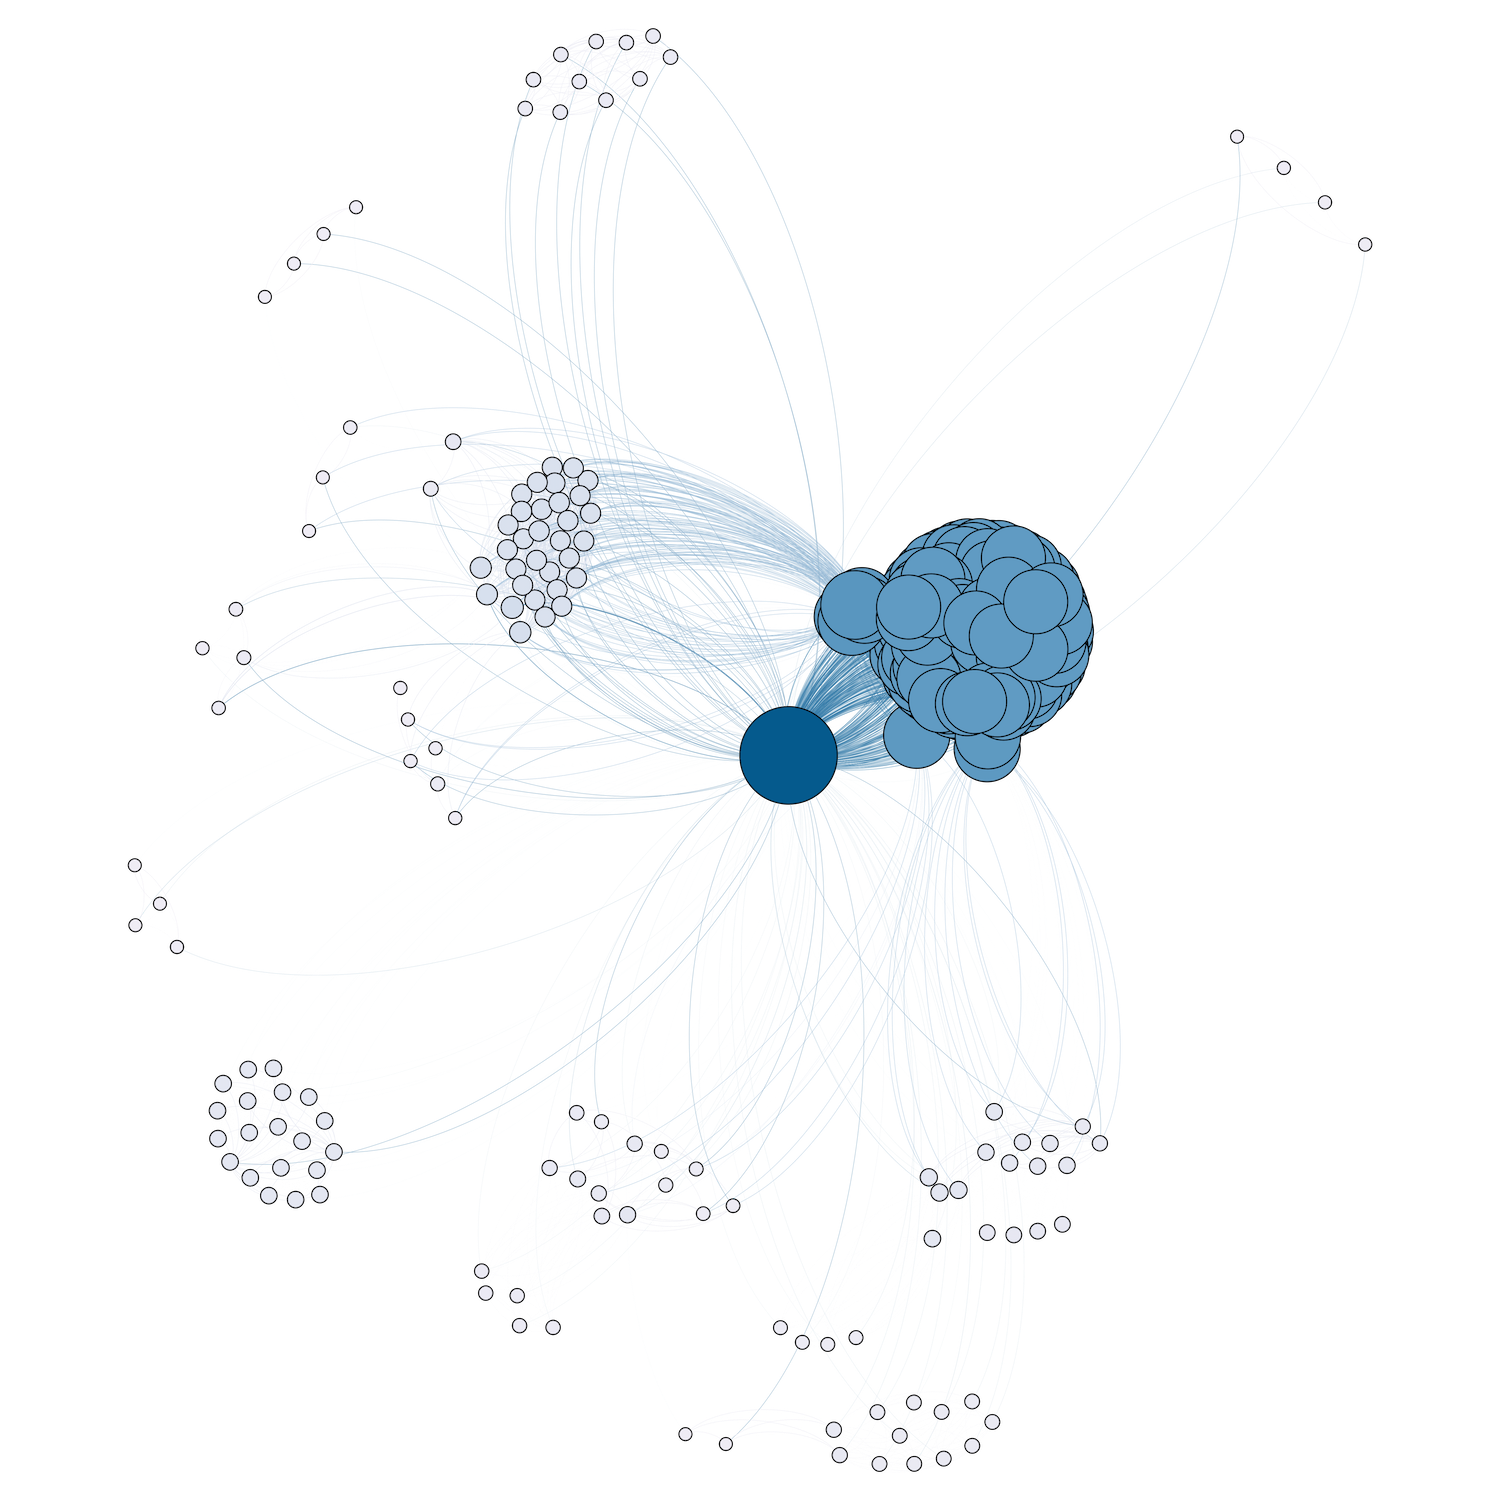
\includegraphics[width=\textwidth]{figures/kostas_descriptive.png}
		\caption{\textsf{Konstantinos Xirogiannopoulos (small)}}
        \label{fig:kostas_descriptive}
	\end{subfigure}
    \caption{\textsf{Email networks, no matter the size are complex.}}
    \label{fig:descriptive}
\end{figure}

As shown in Figure \ref{fig:descriptive}, the authors have elected to use their personal email networks, and through a simple initial visualization it becomes clear that email networks are large and complex.  The nodes in these networks represent the unique email addresses of the individuals who are participating in email communications, and the edges indicate a relationship via email, that is that both email addresses were included together in some email. Edge weights on the graph indicate the frequency of combined participation between two email addresses, the more frequent two email addresses are together on the same email, the stronger the weight. Table \ref{tab:network_comparision} gives descriptive statistics on the relative sizes of these two networks.

\begin{table}[t!]
    \centering
    \label{tab:network_comparison}
    \begin{tabular}{l | c c}
        \hline
        Metric & Benjamin & Kostas \\
        \hline
        Emails & 52,716 & 9879 \\
        Nodes & 3,408 & 1,005 \\
        Edges & 37,158 & 56,370 \\
        Avg. Degree & 21.8063 & 112.1791 \\
        \hline
    \end{tabular}
    \caption{Description of Email Datasets}
\end{table}

Although both of these networks are comparable, because Benjamin's network has three times the number of nodes as Kostas' network, we have elected to call it the "large" network. Interestingly, Kostas' "small" network has significantly more edge connections, and is more connected than Benjamin's graph. We found that this had a very large impact on the choice of layout algorithm to use with the graphs. The "large" network responded very well to the Yifan Hu \cite{hu_efficient_2005} layout, which tended to elongate the network and spread nodes apart in clusters. On the other hand, the "small" network was more suitably laid out by the Fruchterman Reingold method \cite{fruchterman_graph_1991}. Note that neither of these medium sized graphs responded well to the Gephi default layout, the Force Atlas 2 Continuous Layout \cite{jacomy_forceatlas2_2014}.

\begin{figure}[h]
	\centering
	\begin{subfigure}{0.49\textwidth}
		\centering
		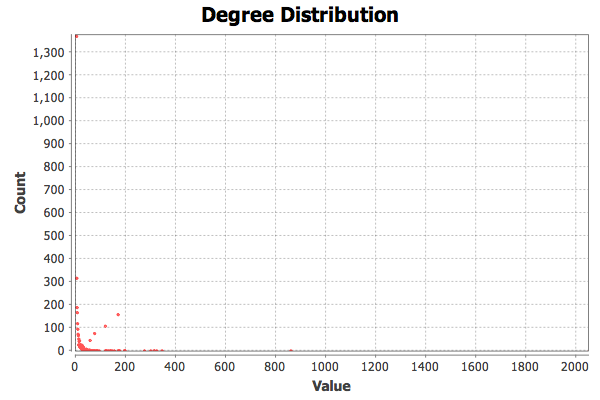
\includegraphics[width=\textwidth]{figures/benjamin_degree.png}
		\caption{\textsf{Benjamin Bengfort (large)}}
        \label{fig:benjamin_degree}
	\end{subfigure} \hfill
	\begin{subfigure}{0.49\textwidth}
		\centering
		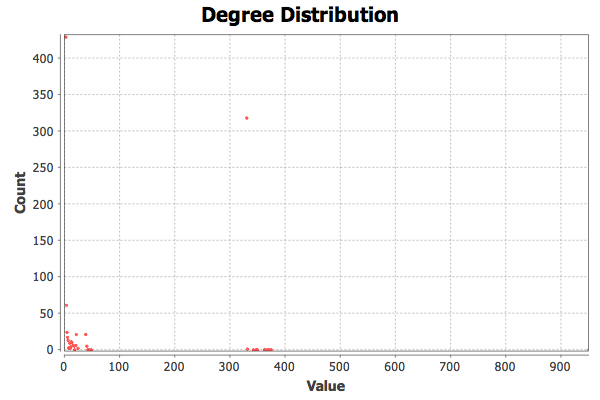
\includegraphics[width=\textwidth]{figures/kostas_degree.png}
		\caption{\textsf{Konstantinos Xirogiannopoulos (small)}}
        \label{fig:kostas_degree}
	\end{subfigure}
    \caption{\textsf{Degree distribution follows a power-laws distribution, common to natural social networks.}}
    \label{fig:degree}
\end{figure}

For the sake of comparison and diversity in our examples, we have extracted both of our email networks, and compared them through several statistical methods. This will allow for more concrete and reliable insight on how network visualization can yield very important insights on vast and complex interconnected data. Importantly, this is possible because both email networks exhibit a power law degree distribution, which is common to social networks and indicates that many desirably human properites can be extracted. The power laws distribution visualization in Figure \ref{fig:degree} was created by Gephi, part of the suite of statistical and reporting tools Gephi is known for.

\subsection*{Data Wrangling for Gephi}

Gephi does not have native Graph extraction tools for social media and email like NodeXL does. Instead, we relied on a tool created by the author called \texttt{tribe}, which is freely available as an open source project\footnote{https://github.com/districtdatalabs/tribe}. The process for extracting a graph from email deserves some attention - as it effects the way that graphs can be visualized. First the email \texttt{mobx} had to be exported from Google using Google's data export tools. The \texttt{tribe} scripts were then used to extract the graph as follows:

\begin{enumerate}
    \item For every email, collect all email addresses regardless of field.
    \item Find all combinations of email address and create edges from combination.
    \item Increment the edge count based on the number of email address combinations
    \item Weight each edge as the frequency of edges across all edges
\end{enumerate}

The \texttt{tribe} tool exported the graph to a GraphML file format, which was easily importable into Gephi. This graph implemented a property graph data structure, and therefore was able to embed more information, for example the domain of the email, or domain frequency. Although these tools weren't used in our particular analysis, it's worth nothing that we had to combine a third-party tool with Gephi in order to get as complete a framework as NodeXL. Even though Gehpi does have a "data laboratory" similar to a spreadsheet, import and export via GraphML was by far the easiest workflow.

\section*{Insights}

% Kostas: Since we have a separate section for the headlines, I don't think this section is necessary. We just talk about the insights in every headline...

% Ben: you're probably right, but an intro paragraph here will make it not look bad, and also the subsection is smaller font, which is better for longer headlines. I leave it up to you, but I think this structure is good.

\begin{figure}[h]
	\centering
	\begin{subfigure}{0.49\textwidth}
		\centering
		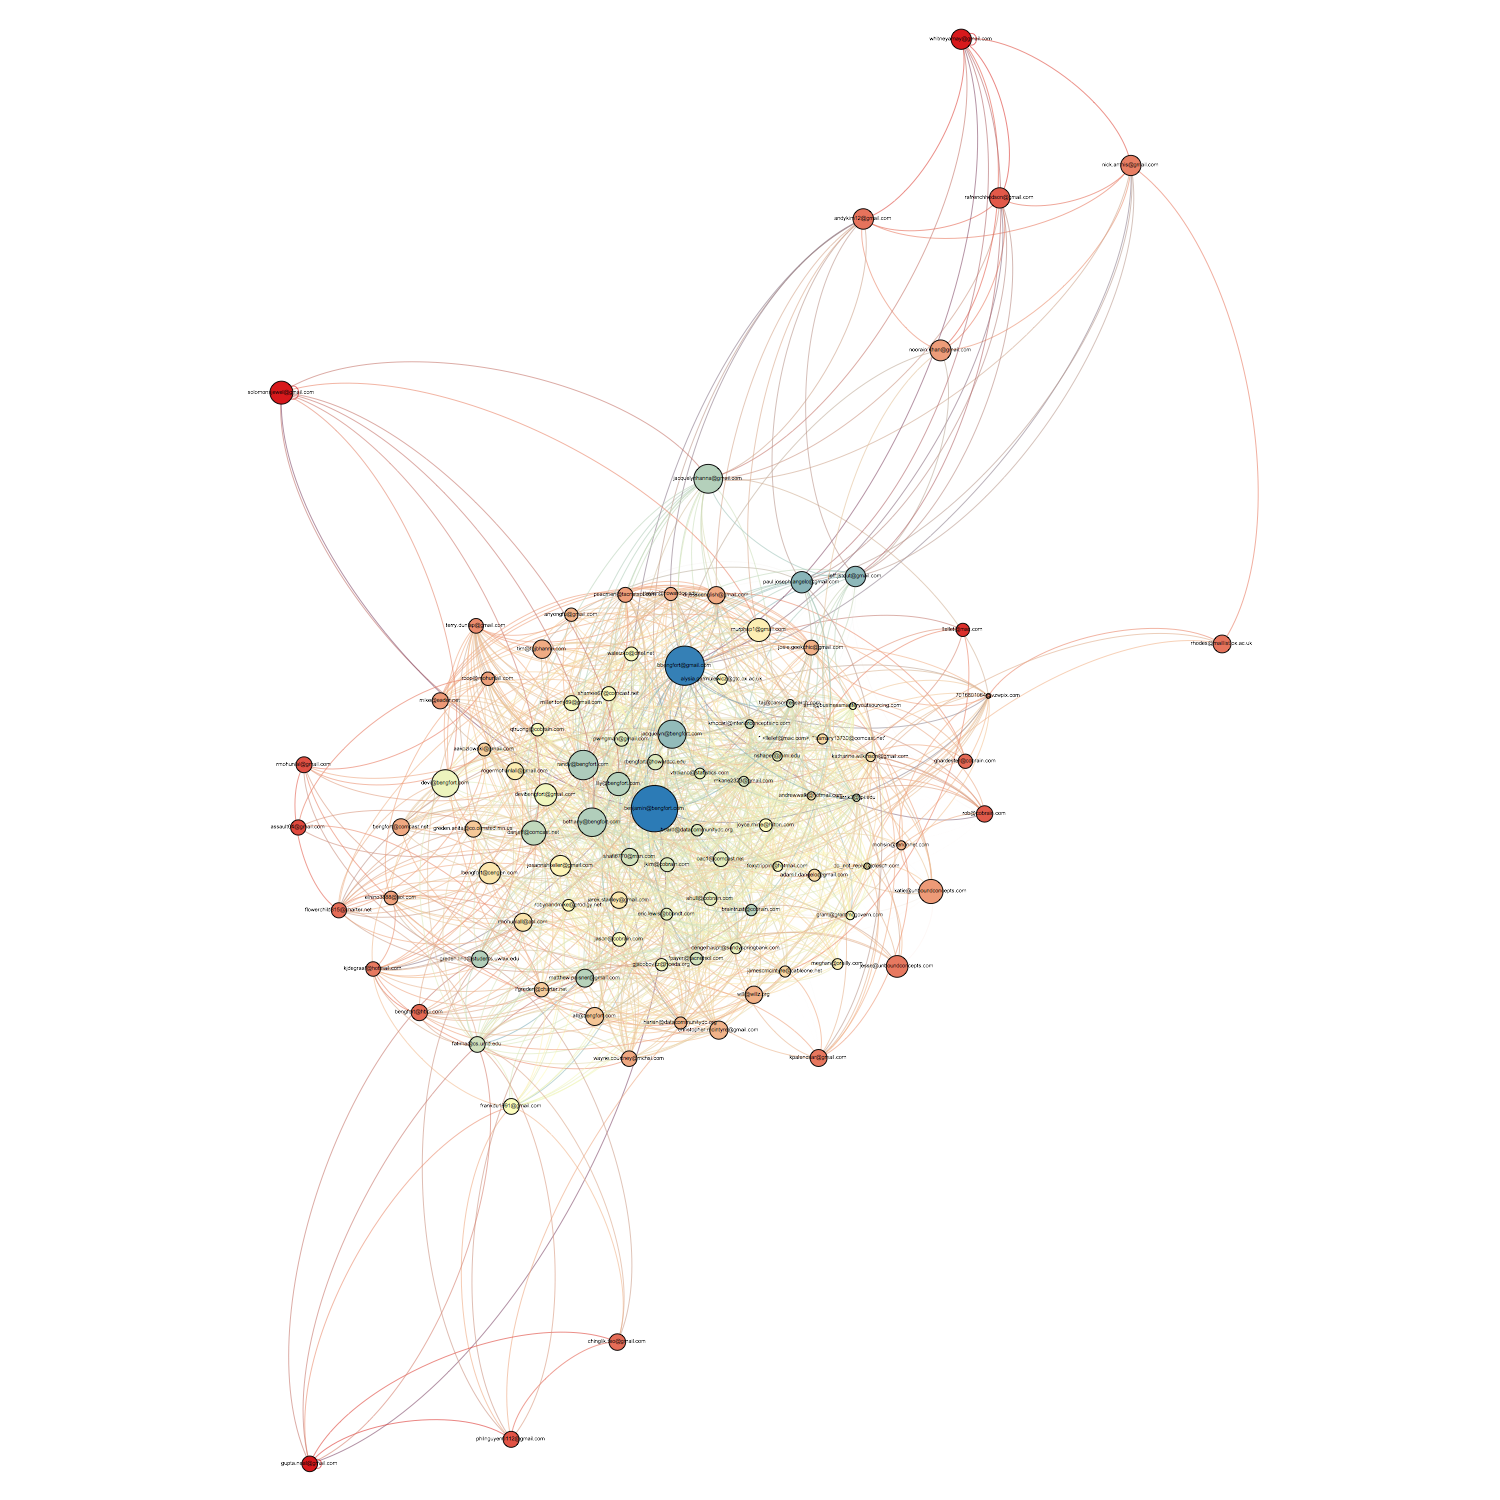
\includegraphics[width=\textwidth]{figures/benjamin_simplification.png}
		\caption{\textsf{Benjamin Bengfort (large)}}
        \label{fig:benjamin_simplification}
	\end{subfigure} \hfill
	\begin{subfigure}{0.49\textwidth}
		\centering
		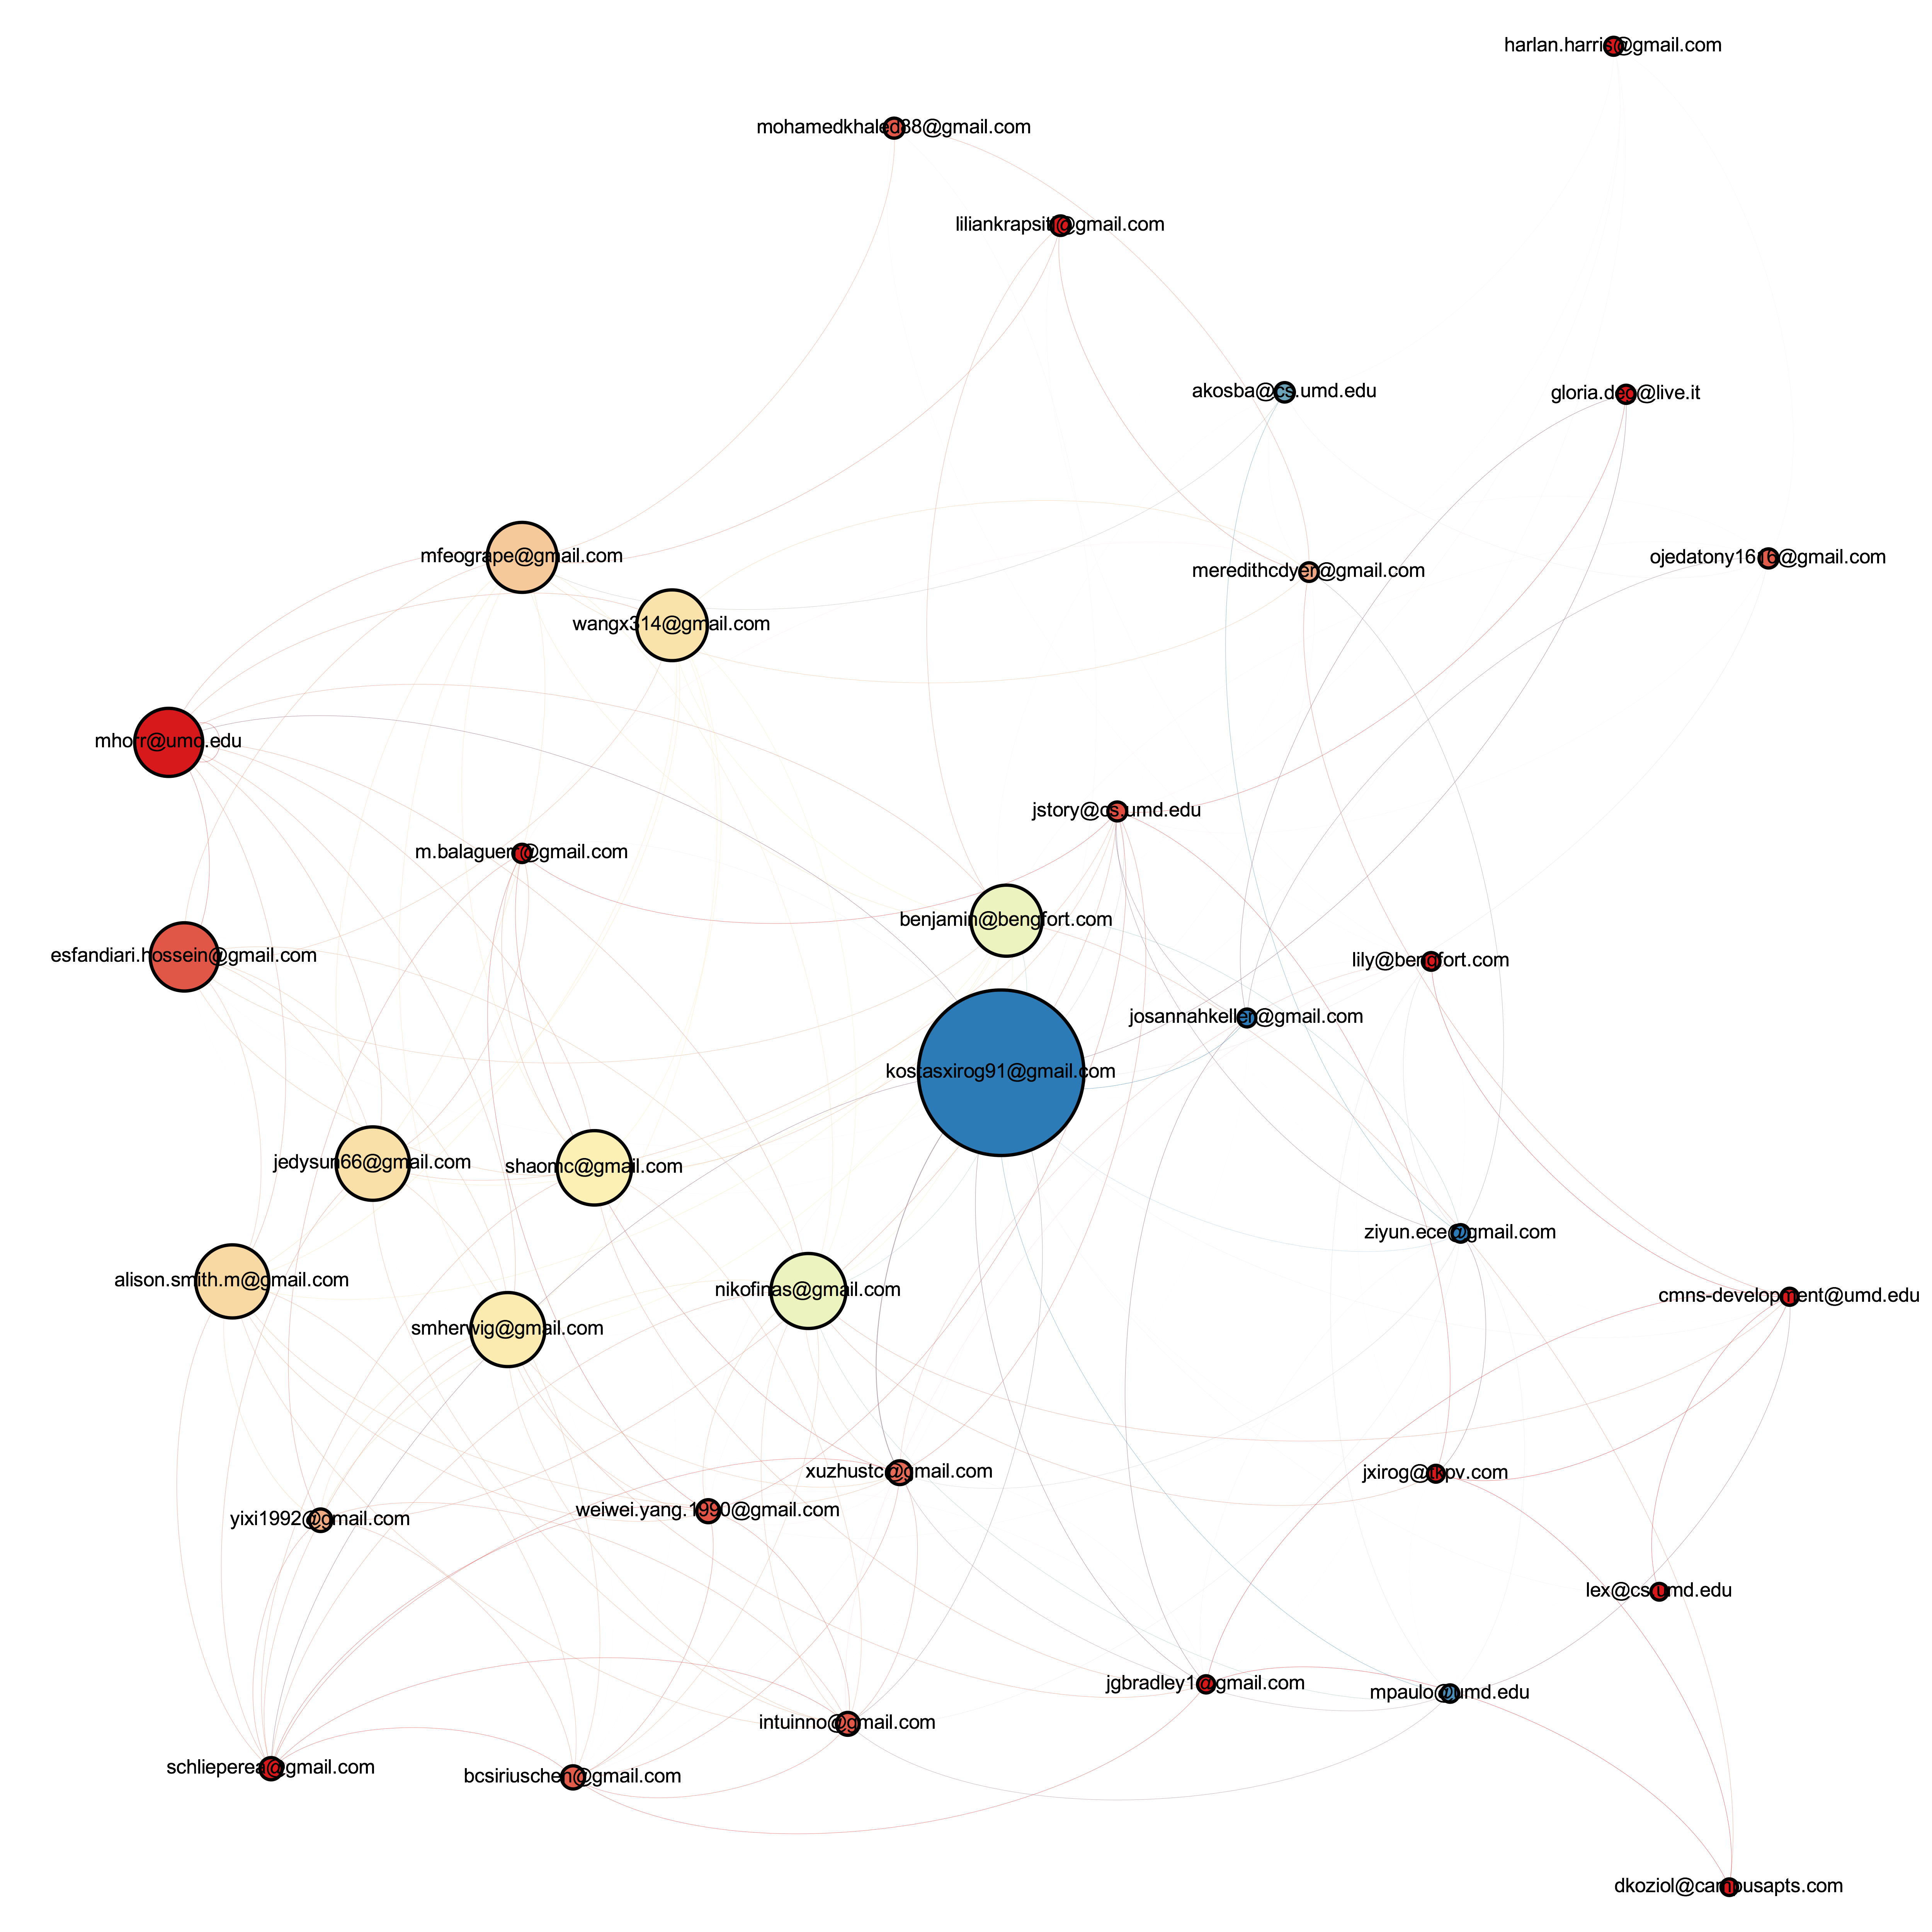
\includegraphics[width=\textwidth]{figures/kostas_simplification.png}
		\caption{\textsf{Konstantinos Xirogiannopoulos (small)}}
        \label{fig:kostas_simplification}
	\end{subfigure}
    \caption{\textsf{Grouping by "Hub" reveals a simpler graph with interesting communication flows.}}
    \label{fig:simplification}
\end{figure}

Our analysis of the large and small email networks was intended to discover central players, communities, and critical communication channels in a visual manner. We explored three techniques for visualization: motif simplification to reduce the complexity of the graph, centrality visualization to identify key players or information channels, and clustering mechanisms to discover communities. The exact same analyses (or steps) were peformed on each email network in sequence, although some minor adjustments were made in layout and formatting to deal with anomalies or peculiarities in individual data sets. However, for the most part, the visualizations listed below can be compared side-by-side as having the same methodology applied to each.

\subsection*{Motif Simplification Reveals Surprising Hubs of Information Flow}

Unfortunately, Gephi does not have the same suite of tools for motif simplification that NodeXL does. Within the Gephi visualization process you can adjust the size, shape, and color of nodes and their labels as well as the color of edges. In order to pursue an analysis similar to "fans" and "connectors" in NodeXL, we instead used a grouping technique to combine similar or highly connected nodes into a single node. We also wanted to find a method to perform edge bundling, a feature reported to be in Gephi \cite{pupyrev_edge_2012,gansner_multilevel_2011}, but were unable to implement it. Figure \ref{fig:simplification} shows how the grouping process can immediately alleviate the complexity of the graph and quickly indicate the most critical hubs of information flow.

Our methodology to simplify the graph was to use a "deduplication" mechanism based on the \texttt{HITS} computation of authority. This methodology computed the node with the highest number of one and two degree triangles within each geodesic. That is- which node is the most connected node in a two degree neighborhood, and also participates in the shortest path. This technique reduced the "large" graph to 61 nodes and the "small" graph to only 29. Because this graph was more managable from a human understanding perspective, this is also the only graph to which we were able to assign labels.

The reduction of nodes was also coupled with some visual motifs. The "authority" of each node was reflected by the size of the node. Furthermore, we used a "betweenness centrality" metric to color the nodes on a continuous gradient scale, where red nodes have a smaller betweenness centrality and blue nodes a larger one. Unfortunately it was impossible to include legends using Gephi, so they were necessarily omitted from the graph.

What was surpising was the nodes that were actually selected as hubs. In both networks the central, most between node is the person whose email inbox we're analyzing, surrounded by green - somewhat between nodes that are critical. However, around the periphery are light yellow and red nodes which act as hubs for more distant (in terms of layout) clusters where email communication is occasional. The hubs in the outer layer are often not ones the authors associate with direct email communications, but rather are often included or CC'd in email messages. This happens so often for a variety of different email conversations and domains (work, school, different sets of friends) that they become more authoritative in the communication process.

\subsection*{Central Nodes Don't Often Have a High Degree}

\begin{figure}[h]
	\centering
	\begin{subfigure}{0.49\textwidth}
		\centering
		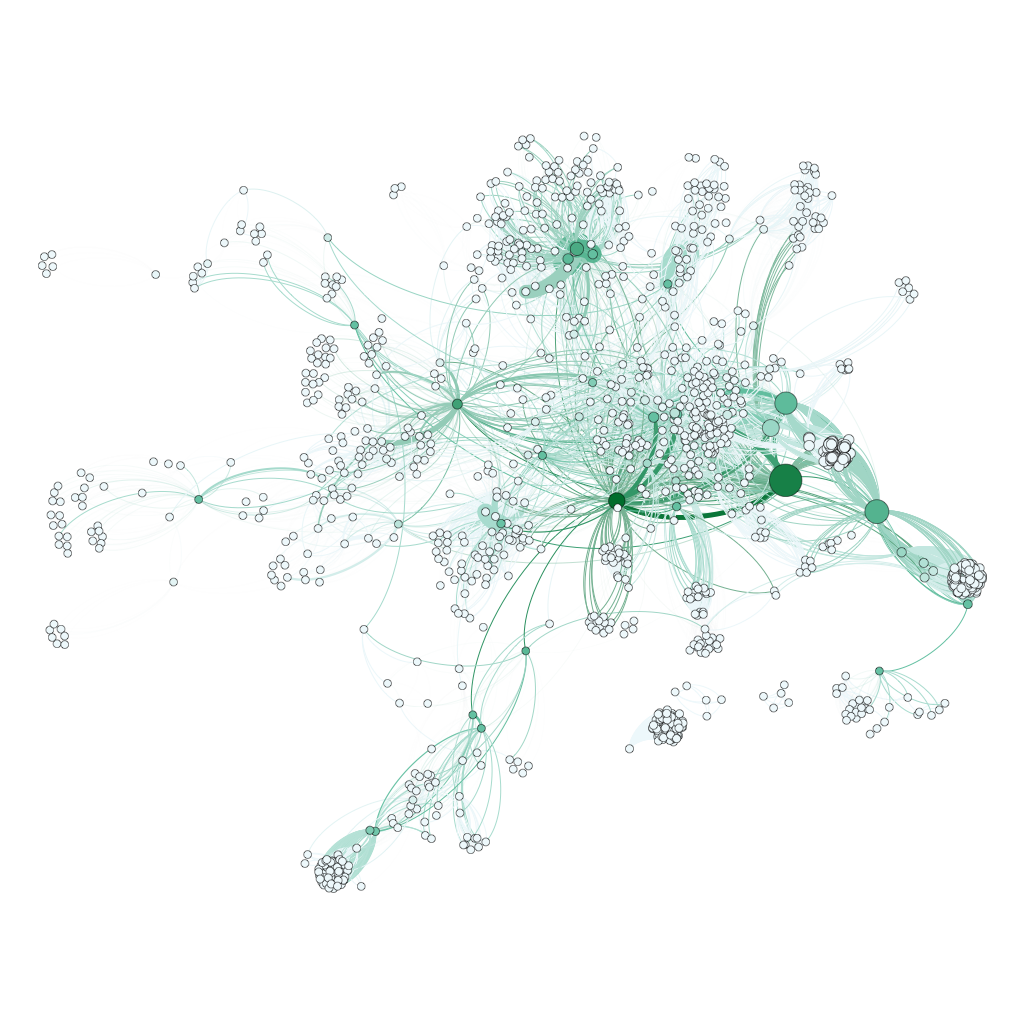
\includegraphics[width=\textwidth]{figures/benjamin_centrality.png}
		\caption{\textsf{Benjamin Bengfort (large)}}
        \label{fig:benjamin_centrality}
	\end{subfigure} \hfill
	\begin{subfigure}{0.49\textwidth}
		\centering
		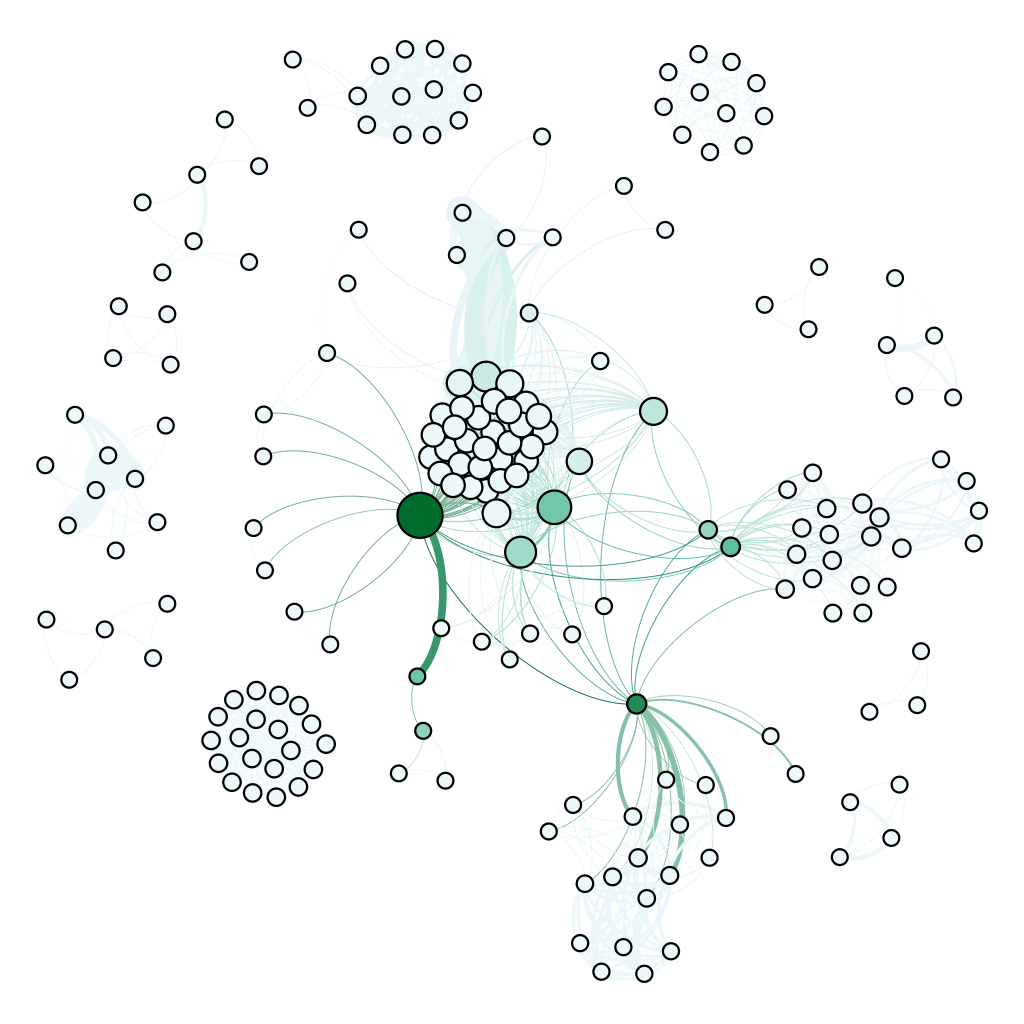
\includegraphics[width=\textwidth]{figures/kostas_centrality.png}
		\caption{\textsf{Konstantinos Xirogiannopoulos (small)}}
        \label{fig:kostas_centrality}
	\end{subfigure}
    \caption{\textsf{Nodes highlighted for their high betweenness centrality}}
    \label{fig:centrality}
\end{figure}

Our next exploration of critical communication channels followed from the idea that surprising nodes had authority because of their degree. Instead, we wanted to include as many nodes as possible and measure their centrality - that is how important they were to the flow of information across the network. In order to simplify the graph without losing too much information, we filtered to ensure only connected nodes to the Giant (the email of the inbox) that had a degree of higher than 4 remained. This removed approximately 60\% of the nodes, but only 10\% of the edges. In order to better visualize key players, the ego node was removed from the visualization.

In Figure \ref{fig:centrality}, the green scale represents the betweenness centrality of each node, where dark green is a high centrality score and white nodes are not central. The size of the node is related to the degree centrality, that is how many edges the node participates in. This graph reveals that the nodes with a high betweenness centrality, that is that they sit on many shortest paths, are often located in critical parts of the graph structurally (e.g. connecting groups), but for the most part do not have a high degree. These "connective" nodes are usually actors who facilitate communication, between one group and another, often directly through the ego node. It is a bit surprising that they shouldn't have a high degree; instead each critical node joins specific subgroups rather than multiple ones.

\subsection*{Revealing Clusters and Communities}
% [Here, we will have our two networks, where we show clusters in them, and compare/contrast the two different networks and the clusters that appear within. I have figured out how to do that and I think it looks cool and will show you my network soon]

\begin{figure}[h]
	\centering
	\begin{subfigure}{0.49\textwidth}
		\centering
		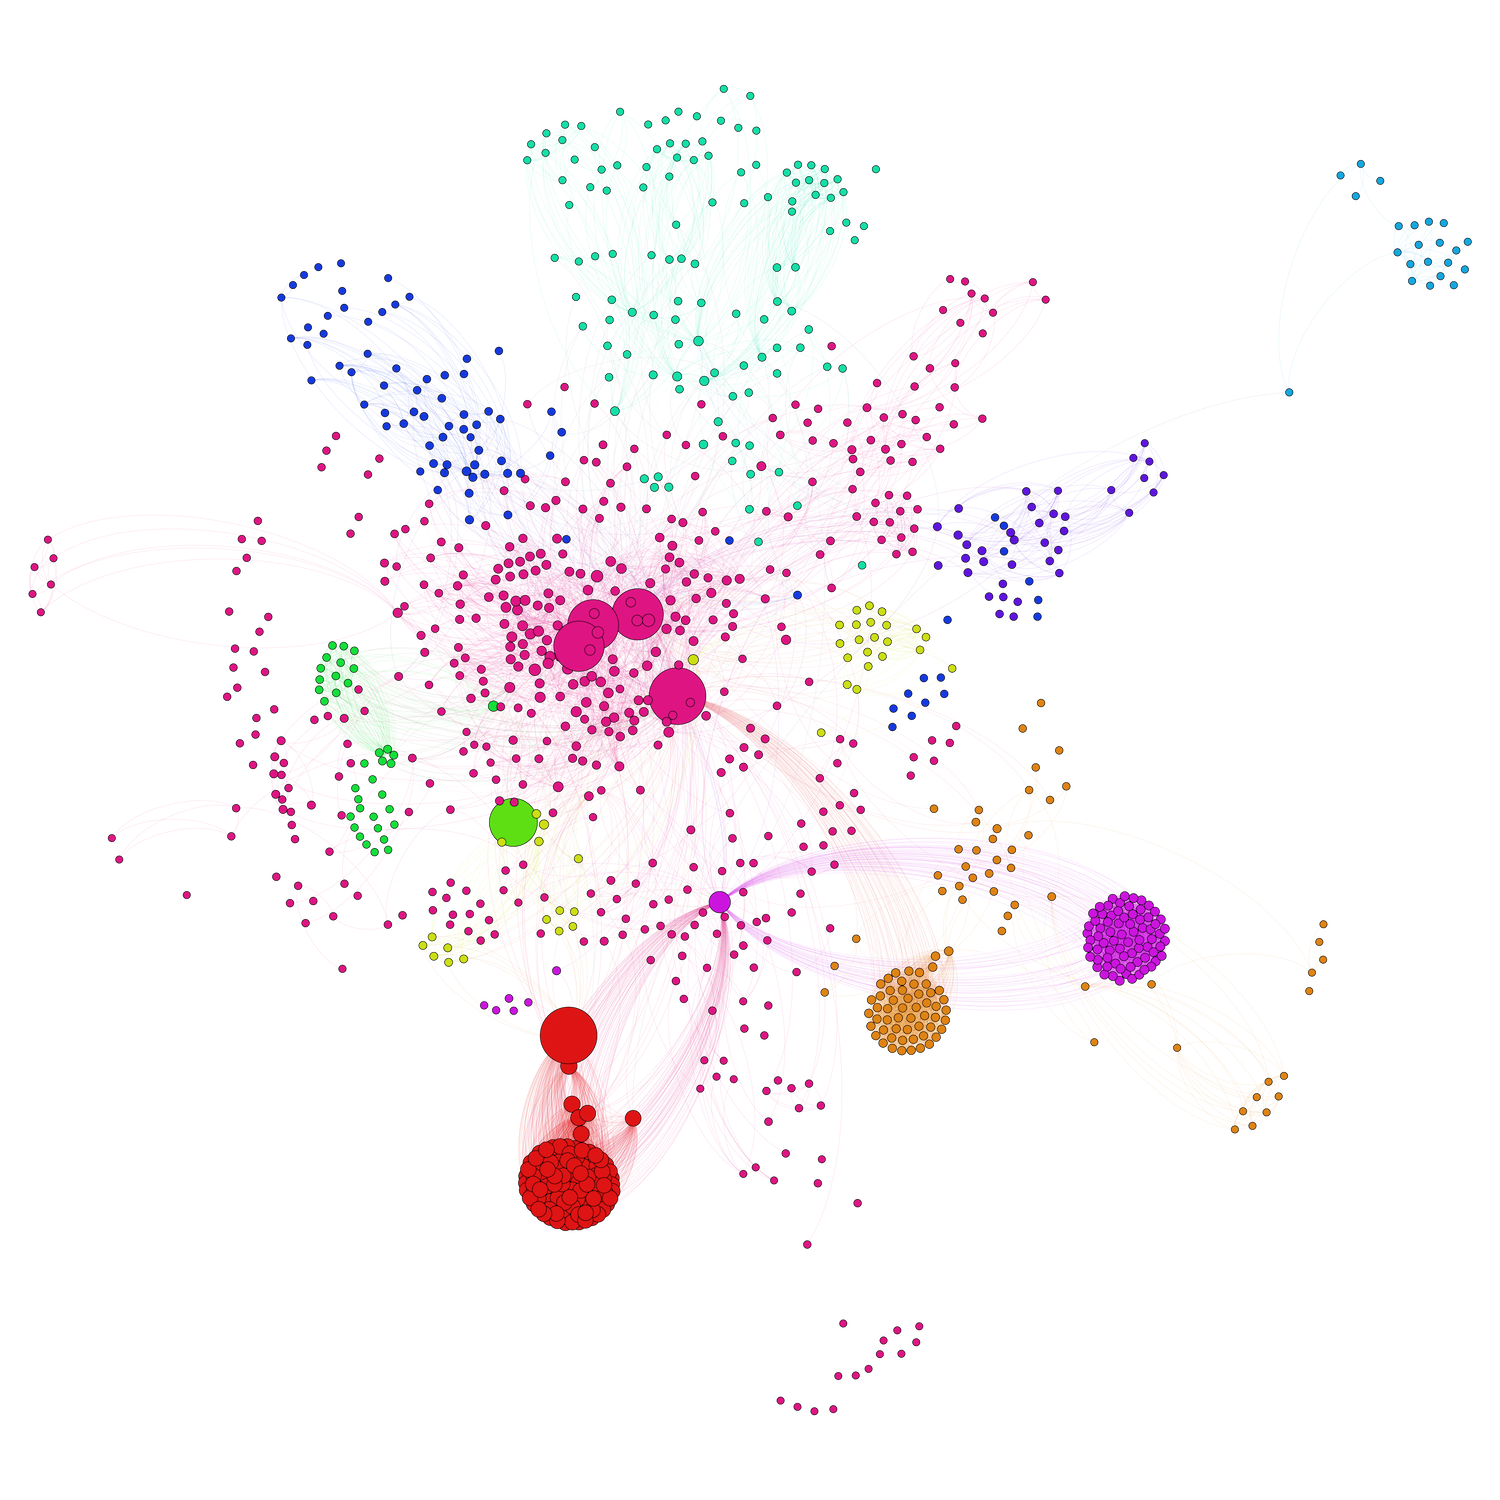
\includegraphics[width=\textwidth]{figures/benjamin_cluster.png}
		\caption{\textsf{Benjamin Bengfort (large)}}
        \label{fig:benjamin_cluster}
	\end{subfigure} \hfill
	\begin{subfigure}{0.49\textwidth}
		\centering
		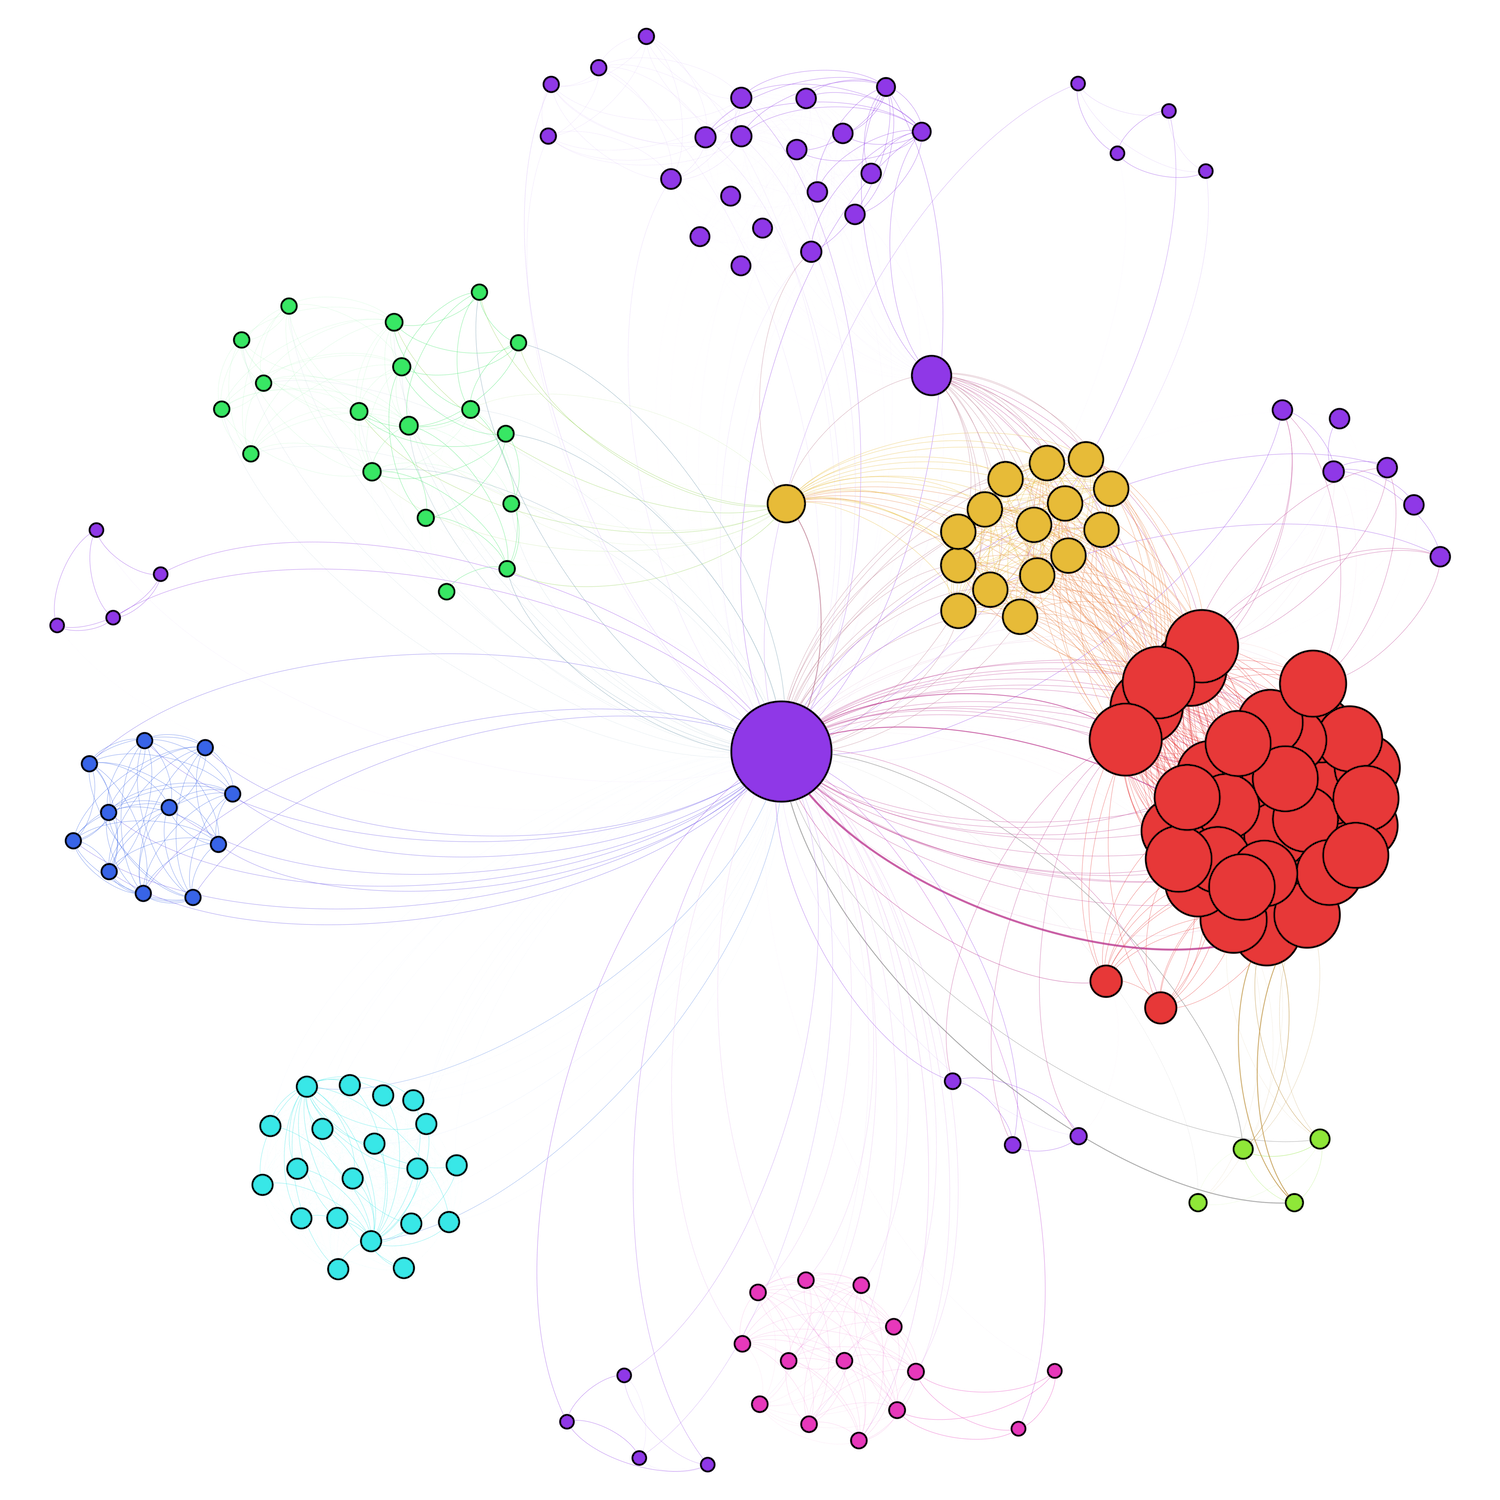
\includegraphics[width=\textwidth]{figures/kostas_cluster.png}
		\caption{\textsf{Konstantinos Xirogiannopoulos (small)}}
        \label{fig:kostas_cluster}
	\end{subfigure}
    \caption{\textsf{Clusters (modularity) colored in email network.}}
    \label{fig:cluster}
\end{figure}

By visualizing our email networks in certain ways, and with the help of some useful features that \textit{Gephi} provides, we were able to extract and reason about about the clusters that form around the center node. To reach this result we used \textit{K-Core filtering} to remove the low degree nodes, as well as \textit{modularity} feature to extract the clusters. As seen in [Figure] there are several clusters that form can form, some of which the center node takes place in, but also some that are disconnected from the center node. Some clusters are very loosely connected, while others share very dense sets of connections. By using the Fruchterman Reingold[] layout algorithm, the clusters appear very clearly and in an organized fashion, around the center node. This layout algorithm allows clusters to emerge and by using \textit{Gephi} we were able to then start digging deeper into what these clusters signify. The emails of our contacts are not shown in the visualization in order to maintain privacy, however \textit{Gephi} allows us to view the email adresses of each node as a label.

Louvian Community Detection \cite{de_meo_generalized_2011}

\subsection*{Small graph}
In the graph on the right, we can clearly make out the clusters that appear in this individual's network. For example, the red cluster is the university email cluster, and includes email that occured during team projects. This cluster is extremely dense, as emails are being sent back and forth between team members, including everyone in the conversation. There are also a few very thick edges in the graph, between the center node and one more node. This signifies vast amounts of email between these two nodes and only between them.


\section*{Critique}

Gephi has some very large pros to it. It is a multi platform tool that can be used for a wide array of graph visualizations. The most important part in visualizing a graph seems to be laying it out properly. \textit{Gephi} has a complete set of layout algorithms that work very well, and allow for laying out the graph in various ways, depending on the size and shape of the graph. \textit{Gephi} also includes various of great \textit{filtering} features, that allow the user to extract a more version of their graph that only includes tha nodes and edges that should be included and that will make sense for the analysis. A wide variety of graph statistics can also effortlessly be computed, and used as parameters in the visualization. Overall, we believe that someone who is already somewhat familiar with \textit{Gephi}, can easily go from raw graph data, to very insightful visualizations in a matter of a few minutes.

Like any tool out there, \textit{Gephi} has a few downsides to it, and unfortunatelly in this case they are critical the the smooth usability of the tool. Firstly, we found several very severe bugs in \textit{Gephi}, for instance when the user saves their progress on a visualization in a .gephi project file, that file then cannot be re-opened, therefore if the program crashes or the user shuts down their computer, they must start from the beginning and re-trace their steps to get the same result. Furthermore, there is no \textbf{undo} functionality in \textit{Gephi}. This is something very unfortunate and makes the tool very difficult to use as the user cannot revert a change that was made by accident. Overall, \textit{Gephi} has a bit of a steep learning curve, before the user understands what each filter and layout does and are able to get their graph down to a manageable size and shape.

Gephi is certainly not as complete as NodeXL - but a dedicated system rather than a tie into Microsoft Excel made it more easily accessible on other platforms.

\section*{Conclusion}

What we did, what we learned, what we'd do again.


\bibliographystyle{plain}
\bibliography{paper}

\end{document}
